\documentclass[12pt]{article}
\usepackage{amsmath}
\usepackage{array}
% \usepackage{gensymb}
\usepackage{geometry}
\usepackage{graphicx}
\usepackage{pgfplots}
\usepackage{siunitx}
\usepackage{wrapfig}

\title{Homework \#3, 4B}
\author{Donald Aingworth IV}
\date{February 5, 2025}

\pgfplotsset{width=8cm,compat=1.9}
\usepgfplotslibrary{external}
% \tikzexternalize

\begin{document}

\DeclareSIUnit{\mile}{mi}
\DeclareSIUnit{\gal}{gal}
\DeclareSIUnit{\foot}{ft}
\DeclareSIUnit{\hour}{h}
\DeclareSIUnit{\rad}{rad}
\DeclareSIUnit{\unit}{u}
\DeclareSIUnit{\dyne}{dyn}

\maketitle

\pagebreak
\section{Question 1}
Figure 22-22 shows three arrangements of electric field lines. In each arrangement, a proton is released from rest at point A and is then accelerated through point B by the electric field. Points A and B have equal separations in the three arrangements. Rank the arrangements according to the linear momentum of the proton at point B, greatest first.\\
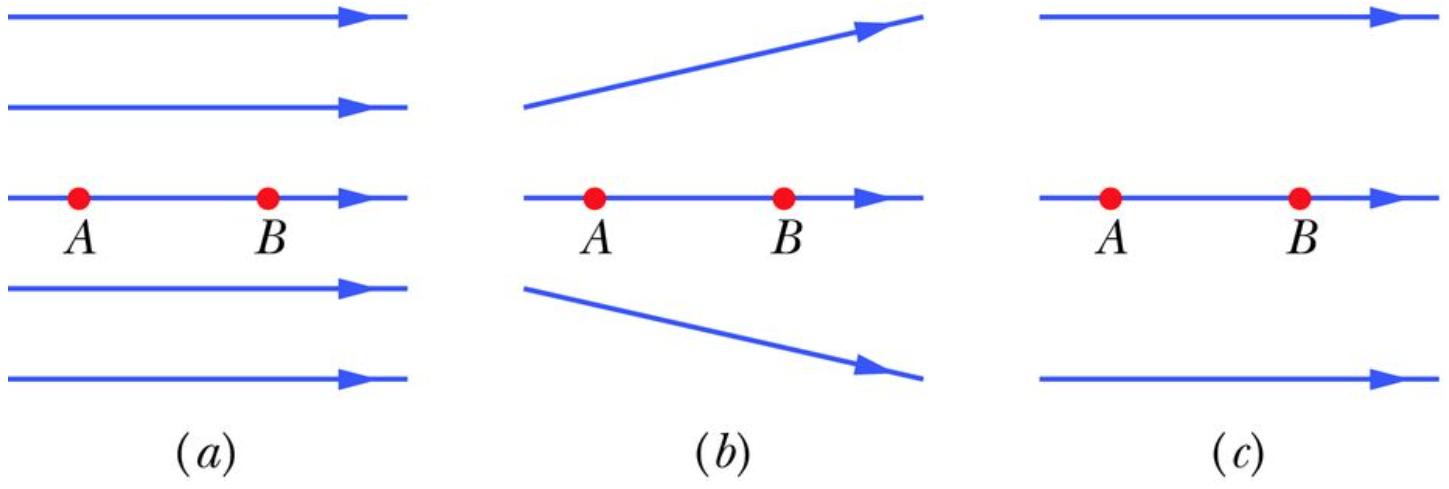
\includegraphics[width=\textwidth]{picture_1.png}

\subsection*{Solution}


\pagebreak
\section{Question 6}
\begin{wrapfigure}{r}{0.5\textwidth}
    \vspace{-30pt}
    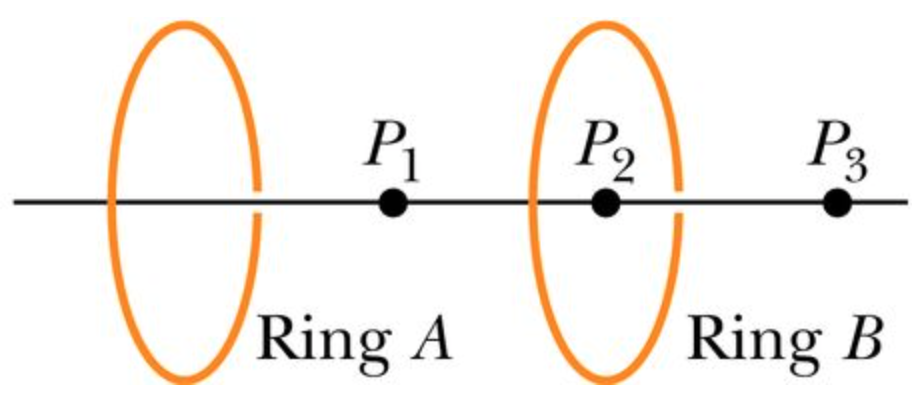
\includegraphics[width=0.5\textwidth]{picture_2.png} 
    % \label{fig:wrapfig}
\end{wrapfigure}
In Fig. 22-27, two identical circular nonconducting rings are centered on the same line with their planes perpendicular to the line. Each ring has charge that is uniformly distributed along its circumference. The rings each produce electric fields at points along the line. For three situations, the charges on rings $A$ and $B$ are, respectively, (1) $q_0$ and $q_0$, (2) $-q_0$ and $-q_0$, and (3) $-q_0$ and $q_0$. Rank the situations according to the magnitude of the net electric field at (a) point $P_1$ midway between the rings, (b) point $P_2$ at the center of ring B, and (c) point $P_3$ to the right of ring B, greatest first.

\subsection*{Solution}


\pagebreak
\section{Question 9}
\begin{wrapfigure}{r}{0.5\textwidth}
    \vspace{-30pt}
    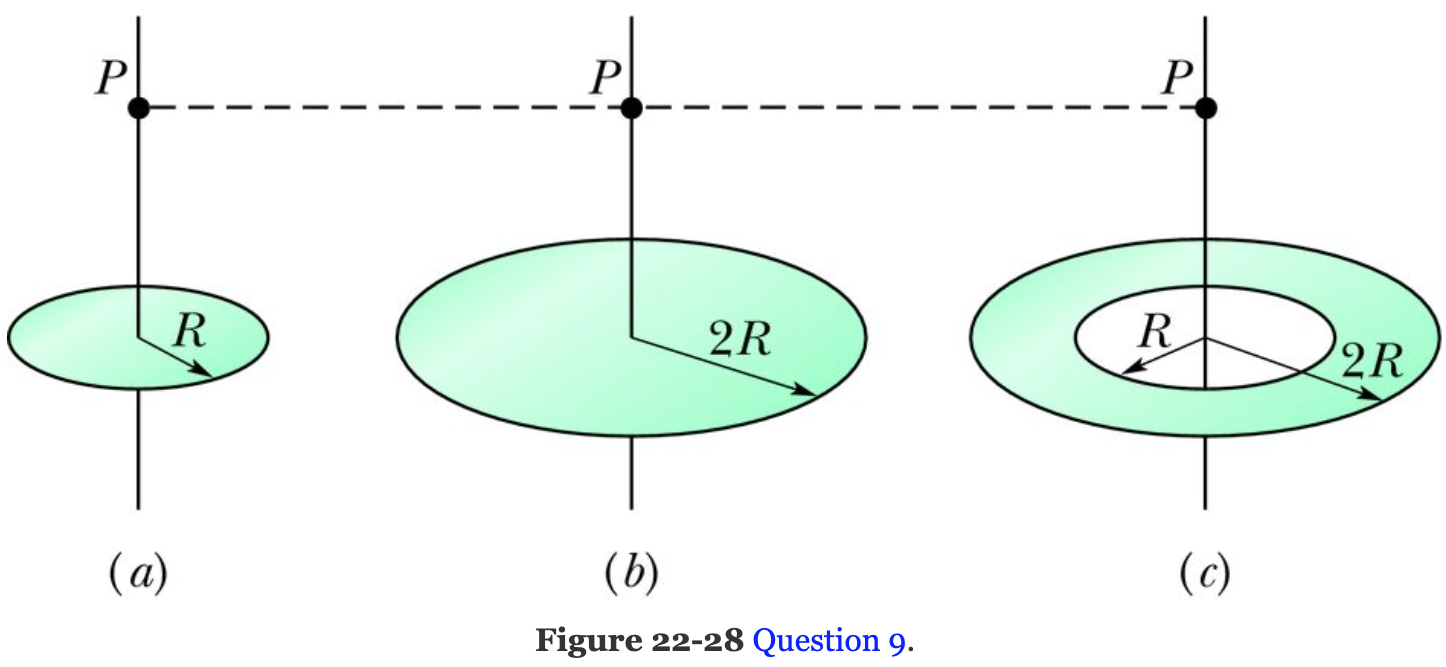
\includegraphics[width=0.5\textwidth]{picture_3.png} 
    % \label{fig:wrapfig}
\end{wrapfigure}
Figure 22-28 shows two disks and a flat ring, each with the same uniform charge Q. Rank the objects according to the magnitude of the electric field they create at points $P$ (which are at the same vertical heights), greatest first.

\subsection*{Solution}


\pagebreak
\section{Question 13}
\begin{wrapfigure}{r}{0.5\textwidth}
    \vspace{-30pt}
    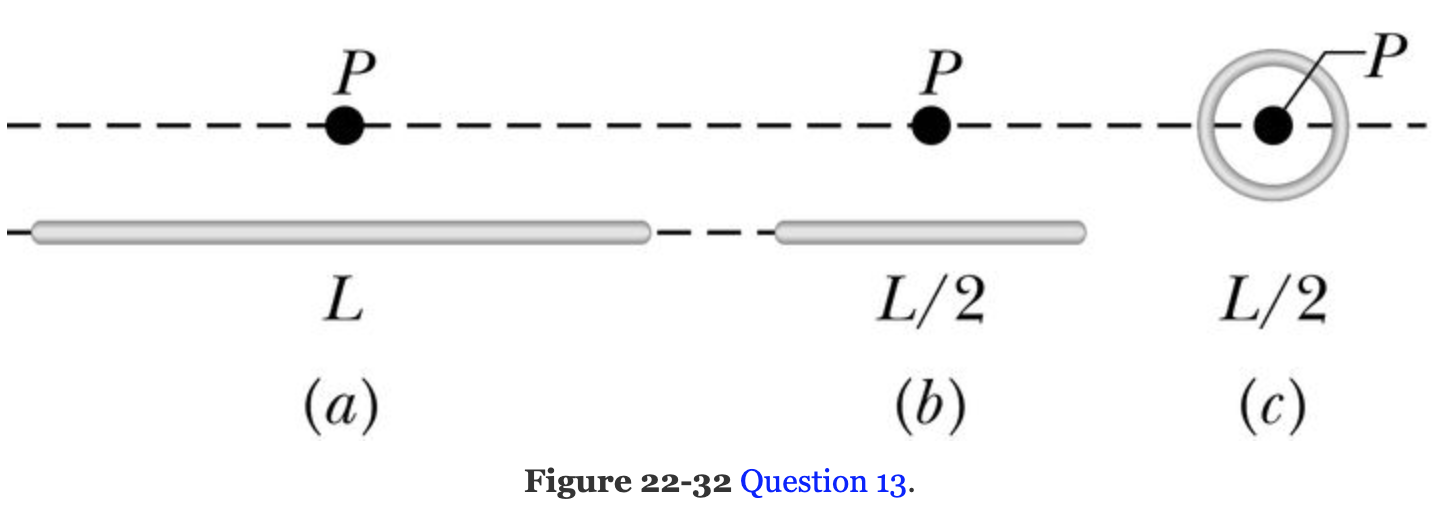
\includegraphics[width=0.5\textwidth]{picture_4.png} 
    % \label{fig:wrapfig}
\end{wrapfigure}
Figure 22-32 shows three rods, each with the same charge Q spread uniformly along its length. Rods $a$ (of length $L$) and $b$ (of length $\frac{L}{2}$) are straight, and points $P$ are aligned with their midpoints. Rod c (of length $\frac{L}{2}$) forms a complete circle about point $P$. Rank the rods according to the magnitude of the electric field they create at points $P$, greatest first.

\subsection*{Solution}


\pagebreak
\section{Problem 24}
\begin{wrapfigure}{r}{0.35\textwidth}
    \vspace{-30pt}
    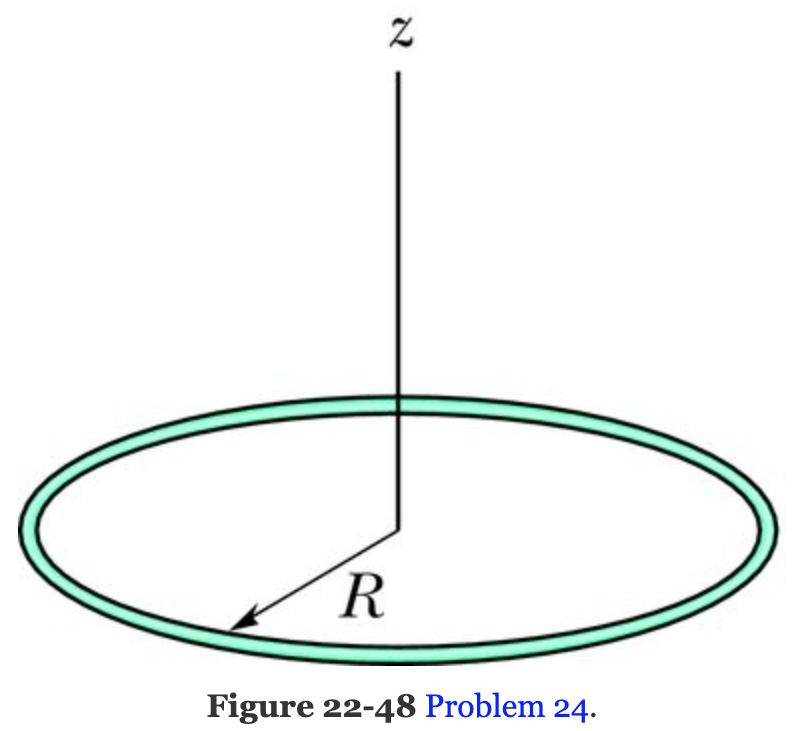
\includegraphics[width=0.35\textwidth]{picture_5.png} 
    % \label{fig:wrapfig}
\end{wrapfigure}
A thin nonconducting rod with a uniform distribution of positive charge Q is bent into a complete circle of radius R (Fig. 22-48). The central perpendicular axis through the ring is a z axis, with the origin at the center of the ring. What is the magnitude of the electric field due to the rod at (a) z = 0 and (b) z = $\inf$? (c) In terms of R, at what positive value of z is that magnitude maximum? (d) If R = 2.00 cm and Q = 4.00 C, what is the maximum magnitude?

\subsection*{Solution}


\pagebreak
\section{Problem 26}
\begin{wrapfigure}{r}{0.5\textwidth}
    \vspace{-30pt}
    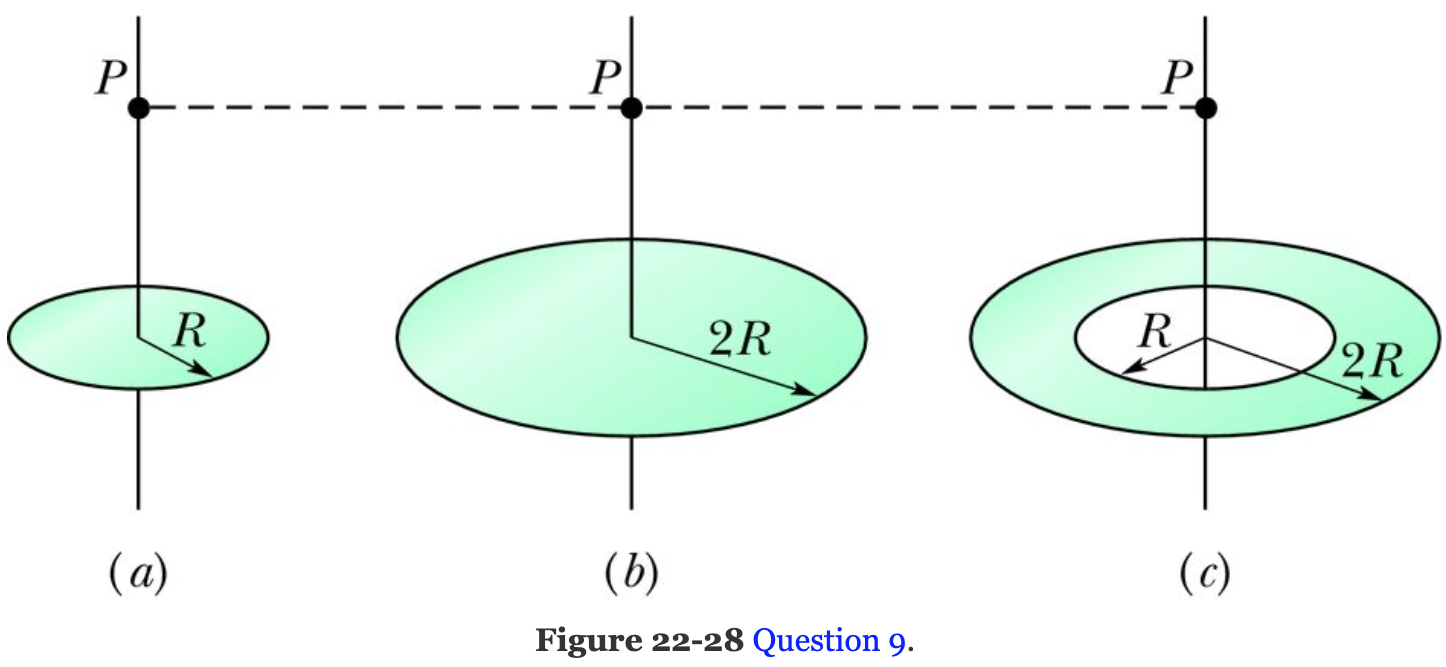
\includegraphics[width=0.5\textwidth]{picture_3.png} 
    % \label{fig:wrapfig}
\end{wrapfigure}
Fig. 22-50, a thin glass rod forms a semicircle of radius $r = 5.00 \unit{\centi\meter}$. Charge is uniformly distributed along the rod, with $+q = 4.50 \unit{\pico\coulomb}$ in the upper half and $-q = -4.50 \unit{\pico\coulomb}$ in the lower half. What are the (a) magnitude and (b) direction (relative to the positive direction of the x axis) of the electric field E at P, the center of the semicircle?

\subsection*{Solution}


\end{document}